
\labtitle{\semester}{Master Theorem}{TBD}

\section*{Learning Goals}
During this lab, you will:
\begin{itemize}
    \item review the Simplified Master Theorem
    \item solve recurrences by iteration and using the S.M.T.
    \item identify recurrences that can not be solved using the S.M.T.
\end{itemize}

\section*{Simplified Master Theorem}

The \textbf{master theorem} is a powerful tool in the analysis and classification of recurrences. It may be used to easily \textit{classify} recurrences that might otherwise be very time-consuming!

\begin{framed}
    \begin{center}\underline{Simplified Master Theorem}\end{center}
    Given a recurrence $T(n)$ of the form,
    $$
        T(n) = \left\{
        \begin{array}{lr}
            c & n < c_1\\
            a T(n/b) + \Theta(n^i) & n \geq c_1
        \end{array}\right.
    $$

    Case I: If $a > b^i$ then $T(n) = \Theta(n^{\log_b a})$.\\

    Case II: If $a = b^i$ then $T(n) = \Theta(n^i \log_b n)$.\\

    Case III: If $a < b^i$ then $T(n) = \Theta(n^i)$.
\end{framed}

This probably seems very magical and hand-wavy. But we're computer scientists, so let's delve in and figure this out. Let us assume here that $n$ is some power of $b$.

\begin{figure}[ht]
    \centering
    
\includegraphics[width=\textwidth*3/8]{harrywizard.png}
    \caption*{\textit{You don't need to be a wizard to understand the master theorem!}}
\end{figure}

\begin{figure}[ht]
    \centering
    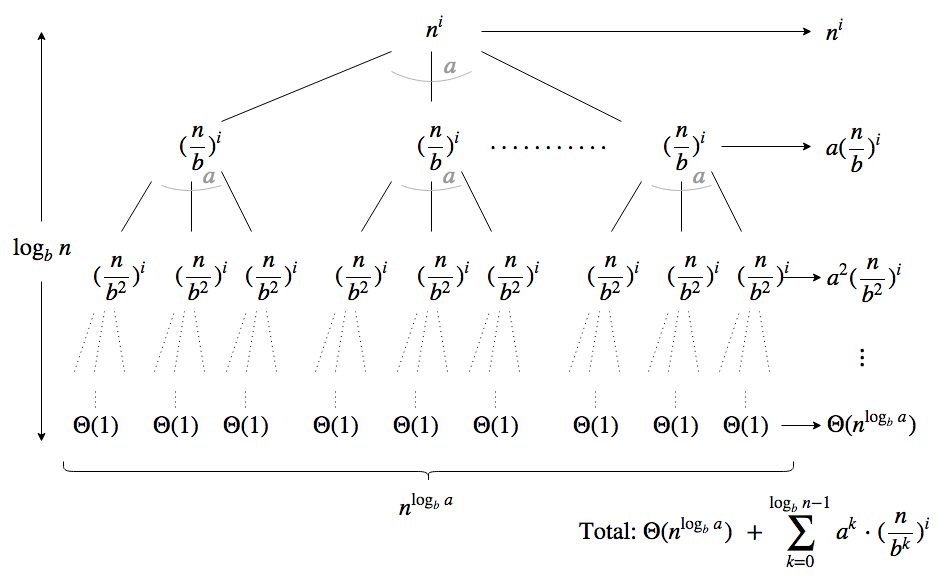
\includegraphics[width=\textwidth*5/8]{master_theorem_tree_1.png}
    \caption*{\textit{Depicted above is a tree-representation of the work performed at each level of iteration in the recurrence.}}
\end{figure}

\subsection*{Understanding the S.M.T.}

To understand why the S.M.T. works, let's draw out the recurrence tree for $T(n)$. \\

As shown in the diagram on the next page, at the $k$th level of iteration, there are $a^k$ subdivisions of $(n/b^k)^i$ work. Therefore, at the bottom-most level there are $a^{\log_b n}$ subdivisions of $(n/b^{\log_b n})^i = 1$ work. Recall that by the properties of logarithms, $a^{\log_b n} = n^{\log_b a}$ --- so we can switch the base and the contents of the log.

We can therefore write the total amount of work represented by the recurrence $T(n)$ as,

$$\text{Total Work: }\Theta(n^{\log_b a}) + \sum_{k=0}^{\log_b{n-1}} a^k\cdot (\frac{n}{b^k})^i$$

So what does this mean in the three cases shown in the simplified master theorem?\\

In the case where $a > b^i$, the work done at the leaves \textit{heavily} outgrows that done at the root. That is, $n^{\log_b a}$ is the dominating term in the sum and the total work is therefore $\Theta(n^{\log_b a})$.\\

In the case where $a = b^i$, the work done at each level is the same and the total work is just the height of the tree multiplied by the work at each level: $\Theta(n^i \log_b n)$.\\

In the case where $a < b^i$, then the work done at each subsequent level decreases with respect to the root, and the work done at the root dominates: $\Theta(n^i)$.\\

Tada! By drawing the recurrence tree and summing the total work performed at each level, we were able to find general expressions for the recurrence solutions for each case of the S.M.T.
\section*{Problems}

